\documentclass[b5paper,opensource]{./template/qyxf-book}
%注意,我修改了模板里的\solve,使其后文字首行缩进两字符

% 这里可以自定义一些命令
\newcommand{\di}[1]{\mathrm{d}#1}
\newcommand{\p}[2]{\frac{\partial #1}{\partial #2}}
\newcommand{\pp}[2]{\frac{\partial ^2 #1}{\partial #2 ^2}}
\newcommand{\dy}[2]{\frac{\di{#1}}{\di{#2}}}
\newcommand{\ddy}[2]{\frac{\mathrm{d} ^2 #1}{\mathrm{d} #2 ^2}}
\newcommand{\zbj}[4]
{
	\draw (0,0) node[below left] {$ O $};
	\draw [->] (#1,0) -- (#2,0) node[right] {$ x $};
	\draw [->] (0,#3) -- (0,#4) node[right] {$ y $};
}


\usepackage{siunitx}%输入角度
\usepackage{color}
\renewcommand{\thefootnote}{\color{red}\arabic{footnote}}%更改脚注格式
\usepackage[version=4]{mhchem}%写化学式
\newcommand{\RNum}[1]{\uppercase\expandafter{\romannumeral #1\relax}}%罗马数字
\newenvironment{mymathfrac}[2]{\left.\raise0.5ex\hbox{$#1$}\! \big\left/ \! \lower0.5ex\hbox{$#2$}\right.}%长斜分数线环境

\begin{document}
\setcounter{chapter}{11}
\chapter{热力学基础}
\section{选择题}
\exercise{1}C

\solve 
等体加热内能增大,A错;

等温过程内能不变,$\Delta E = 0,Q+A>0,Q<0$,B错;

由$PV=nRT,V \uparrow ,$则$ T \uparrow,$则$\Delta E > 0,$又$A<0,$则$Q>0$,C正确;

绝热压缩,$A>0,Q=0,$则$\delta E>0$,D错。

\exercise{2}A

\solve 
由容积不变知为等体过程,则${Q_V} = \nu {C_V}({T_2} - {T_1})$,$H_2$为双原子分子,${C_V} = \frac{5}{2}R,$ \ce{NH3}为多原子分子,$C_V=3R$ (本章未提及),则A正确。


\exercise{3}B

\solve 由图中ab及cd围成面积知$\Delta {E_{ab}} = \Delta {E_{cd}},A_{ab} < {A_{cd}},$由$\Delta E = Q + A$知$Q_{ab} > {Q_{cd}},$又${Q_{ab}} = 0,$所以${a_{cb}} < 0,$  即$C < 0,$ 故选B。


\exercise{4}D

\solve 等温:$\delta T=0$

等压:由$PV=nRT,\frac{V_2}{V_1}=\frac{T_2}{T_1} \Rightarrow |\delta T|=T_1$

绝热:由$TV^\gamma=C_2$知$(\frac{V_1}{V_2})^{\gamma-1}=\frac{T_2}{T_1}\rightarrow |\delta T|=|[1-(\frac{1}{2})^{\gamma-1}]T_1|$

则选D。

\exercise{5}D

\solve 绝热线与等温线只有一个交点,A错;

由$PV=nRT$,两者内能变化量相同,但做功不同,则吸热量不同,B错;

曲线下围成面积不同,C错;

由$PV=nRT$,D对。

\exercise{6}D

\solve 等压过程,系统对外做功$A=\nu R(T_2-T_1)$,吸热$Q_P=\nu C_P(T_2-T_1)$,则$\frac{W}{Q}=\frac{A}{Q_P}=\frac{R}{C_P}=\frac{1}{1+\frac{5}{2}}=\frac{2}{7}$

故选D。

\exercise{7}C

\solve $\eta=1-\frac{T_1}{T_2}$,易知BCC'和ADD'分别为等温线,则$\eta_1=\eta_2$;由图,BCD下面积小于BCD',则$W_1<W_2$,故选C。

\exercise{8}C

\solve 体积增大,则W>0;

$T_a=\frac{2p_1V_1}{nR}=T_b$,则$\Delta E=0$,故选C。

\exercise{9}B

\solve A错,绝热斜率应该比等温线绝对值大;

B合理;

C绝热线不能相交;

D同C。

故选B。

\exercise{10}D

\solve 假设可行,则$\eta=1000/1600=62.5\%$,

而由卡诺循环,$\eta=1-\frac{T_2}{T_1}=25\%$,故选D。

\section{计算题}
\exercise{11}$\frac{1}{2}(\frac{C}{V_1}^2-\frac{C}{V_2}^2)$\qquad 减少\qquad 放热

\solve $W = \int_{{V_1}}^{{V_2}} {pdV = } \int_{{V_1}}^{{V_2}} {\frac{C}{{{V^3}}}dV = }  - \frac{1}{2}(\frac{C}{{{V_2}^2}} - \frac{C}{{{V_1}^2}})$

由$PV = nRT,P{V^3} = C$得$T=\frac{C}{nRV^2}$,V增加,T减少,则气体内能减少

$\Delta E = \nu {C_V}({T_2} - {T_1}) = \frac{{{C_V}({p_2}{V_2} - {p_1}{V_1})}}{R} = \frac{{{C_V}}}{R}(\frac{C}{{{V_2}^2}} - \frac{C}{{{V_1}^2}})$

$\Delta Q = \Delta  + A = (\frac{{{C_V}}}{R} - \frac{1}{2})(\frac{C}{{{V_2}^2}} - \frac{C}{{{V_1}^2}}) < 0$

所以放热。

\exercise{12}不重合\qquad$\gamma$不同\qquad 不重合

\solve
$\gamma$不同则其函数型$pV^\gamma=C$不同。

\exercise{13}500\qquad700

\solve 
等压过程中,$A=p\Delta V=\nu \Delta T$,单原子分子$C_{P1}=\frac{5}{2}R$

$Q_1=\nu C_{P1} \Delta T=\dfrac{5}{2}A=500\mathrm{J}$

$Q_2=\nu C_{P2} \Delta T=\dfrac{7}{2}A=700\mathrm{J}$

\exercise{14}温度\qquad 过程\qquad 做功\qquad 传递热量

\exercise{15}2/3\qquad$2S_1$

\solve
$\eta =1-\frac{T_0}{3T_0}=\frac{2}{3}$

$W=\frac{S_1}{1-\eta}-S_1=2S_1$

\exercise{16}1/3\qquad200J

\solve
$\eta =1-\frac{T_2}{T_1}=\frac{1}{3}$

$W=\frac{T_2}{T_1-T_2}=2\mathrm{J}$

$A=\frac{Q_2}{W}=200\mathrm{J}$

\exercise{17}= \qquad >

\solve 两种气体对外做功即为abcda围成的面积,相等。

$\eta=\frac{W}{Q},W$相同,由$pV=nRT$知温度变化量也相同;

ab过程为等压过程,且$C_{I}<C_{II}$,则$Q_{I}<Q_{II}$,则有$\eta_I>\eta_{II}$

\exercise{18}$\frac{1}{2}p_0V_0\qquad 9p_0V_0$

\solve W即为1\to2\to3\to1围成的面积, 易得$W=\frac{1}{2}p_0V_0$

$\Delta E=\nu C_V\Delta T=\frac{3C_Vp_0V_0}{R}=\frac{15p_0V_0}{2}$

对外做功为1\to2下的面积,即$A=\frac{3p_0V_0}{2}$,则$Q=\Delta E+A=9p_0V_0$

\exercise{19}3R

\solve$A=\frac{3p_1V_1}{2}, \Delta E=\nu C_V\Delta T=\frac{3C_Vp_1V_1}{R}=\frac{15p_1V_1}{2}$

$Q=\Delta E+A=9p_1V_1$

$\Delta T=\frac{3p_1V_1}{R} \rightarrow C=\frac{Q}{\Delta T}=3R$

\exercise{20}40J\qquad 120J

\solve 由EBCE循环系统对外做功70J,EDAE过程外界对系统做功30J,则一次循环过程系统对外做净功40J;

由于AEB为绝热过程,则$Q_{EAB}=0$,由$Q=\Delta E+A$知:

$W+\Delta E=Q_{BC}+Q_{CED}+Q_{DA}$

由于理想气体一次循环中的内能不变,则$\Delta=500$,则有$40=-30+Q_{CED}-50$,则
$Q_{CED}=120\mathrm{J}$

又因为CED为等体过程,则$A_{CED}=0,\Delta E=120\mathrm{J}$.

\section{解答题}

\exercise{21}

\solve 由\[Q = \Delta E + A\]

知\[\eta  = 1 - \frac{{\Delta {E_{BC}} + {A_{BC}}}}{{\Delta {E_{DA}} + A{  _{DA}}}}\]
\[{A_{BC}} =  - \frac{1}{2}({p_B} + {p_C})({V_B} - {V_C})\]
\[\Delta {E_{BC}} = \nu {C_V}({T_C} - {T_B}) = \frac{{{C_V}({p_C}{V_C} - {p_B}{V_B})}}{R} = \frac{1}{{\gamma  - 1}}({p_C}{V_C} - {p_B}{V_B})\]
\[ \Rightarrow {Q_{BC}} = \frac{{\gamma  + 1}}{{2(\gamma  - 1)}}({p_C}{V_C} - {p_B}{V_B}) - \frac{1}{2}({p_C}{V_B} - {p_B}{V_C})\]
由于\[\frac{{{p_C}}}{{{V_C}}} = \frac{{{p_B}}}{{{V_B}}}\]
所以\[{p_C}{V_B} = {p_B}{V_C}\]
则\[{Q_{BC}} = \frac{{\gamma  + 1}}{{2(\gamma  - 1)}}({p_C}{V_C} - {p_B}{V_B})\]
同理\[{Q_{DA}} = \frac{{\gamma  + 1}}{{2(\gamma  - 1)}}({p_A}{V_A} - {p_D}{V_D})\]
则\[\eta  = 1 + \frac{{{Q_{BC}}}}{{{Q_{DA}}}} = 1 + \frac{{{T_C} - {T_B}}}{{{T_A} - {T_D}}}\]
在绝热过程AB中\[{T_B}{V_B}^{\gamma  - 1} = {T_A}{V_A}^{\gamma  - 1}\]
\[{p_B}^{\gamma  - 1}{T_B}^{ - \gamma } = {p_A}^{\gamma  - 1}{T_A}^{ - \gamma }\]
则有\[{T_B}^{\gamma  + 1}{(\frac{{{V_B}}}{{{p_B}}})^{\gamma  - 1}} = {T_A}^{\gamma  + 1}{(\frac{{{V_A}}}{{{p_A}}})^{\gamma  - 1}}\]
则\[\frac{{{T_B}}}{{{T_A}}} = \sqrt[{\gamma+1}]{{{{\left(\frac{V_A/p_A}{V_B/p_B}\right)}^{\gamma  - 1}}}} = \sqrt[{\gamma  + 1}]{{{{\left(\frac{V_D/p_D}{V_C/p_C}\right)}^{\gamma-1}}}} = \frac{{{T_D}}}{{{T_C}}}=k\]
则\[\eta  = 1 + \frac{T_C-T_B}{T_A-T_D} = 1 - \frac{T_B}{T_A}\]

\exercise{22}

\solve

(1)
$A = \int_{{V_0}}^{6{V_0}} pdV=7{p_0}{V_0}$

$\Delta E = \nu {C_V}({T_C} - {T_A}) = \frac{{5\nu R({T_C} - {T_A})}}{2} = \frac{5}{2}(6{p_0}{V_0} - 3{p_0}{V_0}) = \frac{{15}}{2}{p_0}{V_0}$

$Q = \Delta E + A = \frac{{29}}{2}{p_0}{V_0}$

(2)
$dS = \frac{{dQ}}{T} = \frac{{dE + pdV}}{T} = \frac{{\nu {C_V}}}{T}dT + \frac{{\nu R}}{V}dV$

\therefore $ \Delta S = \int_{{T_1}}^{{T_2}} {\frac{{\nu {C_V}}}{T}dT + \int_{{V_1}}^{{V_2}} {\frac{{\nu R}}{V}dV}  = } \frac{{5\nu R}}{2}\ln \frac{{6{p_0}{V_0}/\nu R}}{{3{p_0}{V_0}/\nu R}} + \nu R\ln \frac{{6{V_0}}}{{{V_0}}} = 29.29\mathrm{J/K}$

\exercise{23}

\solve
(1)
\begin{figure}[!h]
	\centering
	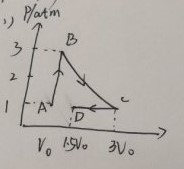
\includegraphics[width=0.35\textwidth]{1.jpeg}
\end{figure}

(2)
\[\frac{{{T_B}}}{{{T_A}}} = \frac{{{p_B}{V_B}}}{{{p_A}{V_A}}} = 3 \Rightarrow {T_B} = 3{T_A} = 900\mathrm{K}\]
\[\nu  = \frac{m}{M} = 0.1\mathrm{mol}\]
\[\Delta {E_1} = \nu {C_V}({T_B} - {T_A}) = 1247.10\mathrm{J}\]
\[\Delta {E_2} = 0\]
\[\Delta {E_3} = \nu {C_V}({T_D} - {T_C}) = 935.3\mathrm{J}\]
则\[\Delta E = \Delta {E_1} + \Delta {E_3} = 311\mathrm{J}\]
\[A = \nu R{T_B}\ln \frac{{3{V_0}}}{{{V_0}}} - \frac{{3P_0V_0}}{2}\]
由${p_0}{V_0} = nR{T_A}$得\[\frac{{3{p_0}{V_0}}}{2} = 374.13\mathrm{J}\]
则\[A = 450.65\mathrm{J}\]
\[Q = \Delta E + A = 762.42\mathrm{J}\]
\exercise{24}

\solve 由下一章知识,\[{C_V} = \frac{i}{2}R,{C_p} = \frac{{i + 2}}{2}R\]
则
\[\gamma=\frac{{i + 2}}{i}\]
因为是绝热过程,则有
\[{T_0}{V_0}^{\gamma-1}={T_\text{\RNum{1}}}{(\frac{V_0}{2})^{\gamma-1}}= {T_\text{\RNum{2}}}{(\frac{{3{V_0}}}{2})^{\gamma-1}}\]
解得
\[{T_\text{\RNum{1}}} = {2^{\frac{2}{i}}}{T_0},{T_\text{\RNum{2}}} = {(\frac{2}{3})^{\frac{2}{i}}}{T_0}\]
则
\[A = \frac{{\nu R}}{{\gamma-1}}({(\frac{2}{3})^{\frac{2}{i}}}{T_0} - {T_0}) + \frac{{\nu R}}{{\gamma  - 1}}({2^{\frac{2}{i}}}{T_0} - {T_0}) = \frac{{i\nu R{T_0}}}{2}[{(\frac{2}{3})^{\frac{2}{i}}} + {2^{\frac{2}{i}}} - 2]\]

\chapter{气体动理论}
\section{选择题}
\exercise{1}B

\solve 微观上,气体温度表示气体分子的运动速度,对于单个或少数分子,温度的概念失去了意义。宏观上,气体的温度表示气体分子的平均冷热程度。

\exercise{2}B

\solve
\begin{gather*} 
{Vp=\sqrt{\frac{2kT}{u}}}\\
{u\left(\ce{O2}\right)}>u\left(\ce{H2}\right)\\
{Vp\left(\ce{O2}\right)<Vp\left(\ce{H2}\right) } \\
\frac{Vp\left(\ce{O2}\right)}{Vp\left(\ce{H2}\right)}=\mymathfrac{\sqrt{\frac{2kT}{32}}} {\sqrt{\frac{2kT}{2}}}=\frac{1}{4}
\end{gather*}
K为常量,T相同。

\exercise{3}C

\solve 自由度为i的分子的平均动能为ikT/2。

\exercise{4}A

\solve

$$
\begin{aligned} \sqrt {\bar{v^{2}}} & = \sqrt { \frac { 3 k T } { u } } \\ u O _ { 2 } & > u H _ { 2 } \\ \sqrt { \bar { v } ^ { 2 } \left( O _ { 2 } \right) } & = \sqrt { \bar { v } ^ { 2 } \left( H _ { 2 } \right) } \\ T \left( O _ { 2 } \right) & > T \left( H _ { 2 } \right) \end{aligned}
$$

\exercise{5}B

\solve 等温过程系统内能不变。

\exercise{6}A

\solve

$$
\begin{array} { c } { \varepsilon _ { H e } = \varepsilon _ { N _ { 2 } } } \\ { n _ { H e } = n _ { N _ { 2 } } \quad n = \frac { N } { V } } \\ { \bar { \varepsilon } = \frac { 3 } { 2 } k T } \\ { T _ { H e } = T _ { N _ { 2 } } } \\ { p = \frac { 2 } { 3 } n \bar { \varepsilon } } \\ { p _ { H e } = p _ { N _ { 2 } } } \end{array}
$$

\exercise{7}A

\solve

$$
\begin{aligned} p V & = \nu R T \\ p V & = \frac { m } { M } R T \\ p V & = \rho R T \\ \rho & = \frac { p M } { R T } \end{aligned}
$$

由于水滴静止,则

$$
p _ { H _ { 2 } } = p _ { O _ { 2 } }
$$

又因为T相同,则

$$
\frac { p _ { H _ { 2 } } } { p _ { O _ { 2 } } } = \frac { \frac { p M _ { H _ { 2 } } } { R T } } { \frac { p M _ { o _ { 2 } } } { R T } } = \frac { 1 } { 16 }
$$

\exercise{8}D

\solve

$$
\begin{aligned} \bar { z } & = \sqrt { 2 } \pi d ^ { 2 } \bar { v } n \\ \lambda & = \frac { 1 } { \sqrt { 2 } \pi d ^ { 2 } n } \end{aligned}
$$

$$
\because n = \frac { p } { k T }
$$不变,$ \bar { v }$不变

$$
\bar { z } = \sqrt { 2 } \pi d ^ { 2 } \bar { v } \frac { p } { k T },p
$$变为原来的两倍

$$
\begin{array} { l } { \therefore z ^ { \prime } = 2 \bar { z } } \\ { \because \bar { v } = \bar { \lambda } \bar { z } } \\ { \therefore \lambda ^ { \prime } = 2 \bar { \lambda } } \end{array}
$$

\exercise{9}C

\solve

$$
\begin{array} { l } { 2 H _ { 2 } O = 2 H _ { 2 } + O _ { 2 } } \\ { E = v \frac { i } { 2 } R T } \end{array}
$$

对于刚性分子,双原子分子气体的i=5,多原子分子气体的i=6

$$
\begin{array} { l } E _ { 0 } = 2 \cdot \frac { 6 } { 2 } R T \\ E _ { 0 } ^ { \prime } = 2 \cdot \frac { 5 } { 2 } R T + \frac { 5 } { 2 } R T = \frac { 15 } { 2 } R T \\ \therefore \frac { 15 } { 2 } R T \div 6 R T = 125 \% \end{array}
$$

\exercise{10}B

\solve

$$
\begin{aligned} \sqrt { \bar { v } ^ { 2 } } & = \sqrt { \frac { 3 k T } { u } } \\ T _ { 2 } & = \frac { 3 } { 2 } T _ { 1 } \\ T _ { 2 } = \left( \frac { 3 } { 2 } \right) ^ { 2 } T _ { 1 } & = 280 \times \frac { 9 } { 4 } = 630 \end{aligned}
$$
\section{填空题}
\exercise{11}
$
\int _ { v _ { 2 } } ^ { v _ { 2 } } f ( v ) N d v
\qquad
\frac { \int _ { v _ { 1 } } ^ { v _ { 2 } } v f ( v ) d v } { \int _ { v _ { 1 } } ^ { v _ { 2 } } f ( v ) d v }
\qquad
N \cdot \frac { 1 } { 2 } m \int _ { v _ { 1 } } ^ { v _ { 2 } } v ^ { 2 } f ( v ) d v
$

\solve
(1)

$$
\begin{aligned} \frac { d N } { N } & = f ( v ) d v \\ d N & = N f ( v ) d v \\ N ^ { \prime } = & \int _ { v_1 } ^ { v _ { 2 } } N f ( v ) d v \end{aligned}
$$

(2)
$$v_1 \sim v_2 \mbox{的平均速度}=\frac{\mbox{这个区间里每个分子速度之和}}{\mbox{这个区间里分子总数}}\\= \frac { \int _ { v _ { 1 } } ^ { v _ { 2 } } v d N } { \int _ { v _ { 1 } } ^ { v _ { 2 } } d N } = \frac { N \int _ { v _ { 1 } } ^ { v _ { 2 } } v f ( v ) d v } { N \int _ { v _ { 1 } } ^ { v _ { 2 } } f ( v ) d v } = \\frac { \int _ { v _ {1 } } ^ { v _ { 2 } } v f ( v ) d v } { \int _ { v _ { 1 } } ^ { v _ { 2 } } f ( v ) d v }$$

(3)
$$\mbox{总平动动能之和=每个分子平动动能之和}= \int _ { v _ { 1 } } ^ { v _ { 2 } } \frac { 1 } { 2 } m v ^ { 2 } d N \\ =  \frac { 1 } { 2 } m N \int _ { v _ { 1 } } ^ { v _ { 2 } } v ^ { 2 } f ( v ) d v 
$$



\exercise{12}$
\frac { N _ { A } } { N _ { A } + N _ { B } } f _ { A } ( v ) + \frac { N _ { B } } { N _ { A } + N _ { B } } f _ { B } ( v )
$

\solve $\frac{N_A}{N_A+N_B}$指的是A在混合气体里占比,B同理



\exercise{13}
$
n _ { 0 } e ^ { - \frac { m g z } { k T } }
\qquad
z = - \frac { k T \ln ^ { \frac { p } { p_0 } } } { m g }
$

\solve 由玻尔兹曼分布律:

$$
\begin{aligned} n & = n _ { 0 } e ^ { - \frac { m g z } { k T } } \\ p & = p _ { 0 } e ^ { - \frac { m g z } { k T } } \\ z & = - \frac { k T \ln ^ { \frac { p } { p _ { 0 } } } } { m g } \end{aligned}
$$



\exercise{14} 升高\qquad 升高

\solve (1)温度应上升。因为高速运动的氧气瓶中的分子是在杂乱无章运动的基础上附加上x方向定向运动速度。氧气瓶静止下来后,气体分子与氧气瓶发生碰撞,高速的x方向定向运动动能通过分子之间的频繁碰撞逐步平均分配到y、z方向的热运动动能上去,所以温度上升。

(2)$pV=\nu RT$,$T$增大,$V,\nu,R$都不变,所以$p$增大。

\exercise{15}$\frac{3kT}{2}$\qquad 温度是大量分子热运动的集体表现,对单个或少数分子来说,温度的概念就失去了意义。

\exercise{16}$
7.82 \times 10 ^ { 7 } s ^ { - 1 } \qquad5 \times 10 ^ { - 5 } \mathrm { cm }
$

\solve

$$
\bar { \lambda } = \frac { k T } { \sqrt { 2 } \pi d ^ { 2 } p }
$$

$\bar { \lambda } $和$\bar { v } $成反比

$$
\begin{array} { l } { p _ { 0 } = 1 \times 10 ^ { 5 } P a } \\ { p _ { 1 } = 1 \times 10 ^ { 4 } P a } \\ { \therefore \overline { \lambda ^ { \prime } } = 10 \bar { \lambda } = 5 \times 10 ^ { - 5 } c m } \\ { z ^ { \prime } = \frac { 1 } { 10 } \bar { z } = 7.82 \times 10 ^ { 7 } s ^ { - 1 } } \end{array}
$$

\exercise{17} 1:4:16\qquad 1:2:4

\solve

$$
\begin{array}{*{20}{c}} \sqrt { \bar { v } ^ { 2 } } = 1.73 \sqrt { \frac { R T } { M } } \\ \because \sqrt { \bar { v } _ { A } ^ { 2 } } : \sqrt { \bar { v } _ { B } ^ { 2 } }  : \sqrt { \bar { v } _ { C } ^ { 2 } } = 1 : 2 : 4 \\ \therefore T _ { A } : T _ { B } : T _ { C } = 1 : 2 ^ { 2 } : 4 ^ { 2 } = 1 : 4 : 16 \\ n = \frac { N } { V } = \frac { \nu N _ { A } } { V } \\ \therefore n \propto \frac { \nu } { V }\\ \therefore \frac { \nu _ { 1 } } { V _ { 1 } } : \frac { \nu _ { 2 } } { V _ { 2 } } : \frac { \nu _ { 3 } } { V _ { 3 } }  = n _ { 1 } : n _ { 2 } : n _ { 3 } = 4 : 2 : 1 \\ p V  = \nu R T \\ p = \frac { \nu R T } { V }  = \frac { \nu } { V } \cdot T \cdot R \\ \therefore p  \propto \frac { \nu } { V } T \\ \therefore p _ { 1 } : p _ { 2 } : p _ { 3 } = 4 \times 1 : 2 \times 4 : 1 \times 16 = 1 : 2 : 4  \end{array}
$$

\exercise{18}6

\solve (1)刚性多原子分子(甲烷)共有6个自由度。

(2)由于分子热运动的无规则性,任何一种运动都不比其他运动占有特别的优越性,所以机会相等,所以分子绕其质心转动对i的贡献为3.

\exercise{19}$
\geqslant 0 
$\qquad 不变 \qquad 增

\solve
(1)孤立系统的熵永远也不会减少。

(2)可逆过程熵不变。

(3)由于ΔS≥0,不可逆过程熵增。


\exercise{20}0 \qquad 增

\solve(1)气体自由膨胀,对外界不做功(A=0)。绝热过程Q=0,ΔE=-A=0。故内能增量为0。

(2)孤立系统的熵永远也不会减少。


\section{计算题}
\exercise{21}

\solve
(1)
\begin{figure}[!ht]
	\centering
	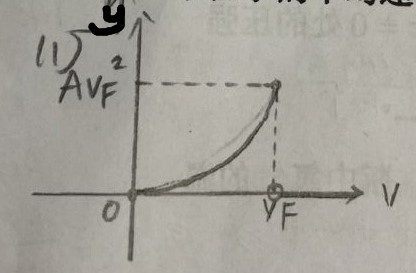
\includegraphics[width=0.35\textwidth]{2_21.jpg}
\end{figure}
\newpage
(2)

$$
\begin{array} { c } { \int _ { 0 } ^ { v _ { F } } A v ^ { 2 } d v = 1 } \\ { \left. \frac { 1 } { 3 } A v ^ { 3 } \right| _ { 0 } ^ { v _ { F } } = 1 } \\ { \frac { 1 } { 3 } A v _ { F } ^ { 3 } = 1 } \\ { A = \frac { 3 } { v _ { F } ^ { 3 } } } \end{array}
$$

(3)

速率分布曲线上与速率分布函数极大值所对应的速率称为最概然速率。

$$ v_P=v_F $$

(4)

$$
\begin{array} { c } { \bar { v } = \int _ { 0 } ^ { v _ { F } } v f ( v ) d v } \\ { \bar { v } = \int _ { 0 } ^ { v _ { F } } v \cdot \frac { 3 } { v _ { F } ^ { 3 } } v ^ { 2 } d v = \left. \frac { 3 } { 4 v _ { F } ^ { 3 } } v ^ { 4 } \right| _ { 0 } ^ { v _ { F } } = \frac { 3 } { 4 } v _ { F } } \end{array}
$$

(5)

$$
\begin{array} { c } { \bar { v } = \int _ { 0 } ^ { v _ { F } } v f ( v ) d v } \\ { \bar { v } = \int _ { 0 } ^ { v _ { F } } v \cdot \frac { 3 } { v _ { F } ^ { 3 } } v ^ { 2 } d v = \left. \frac { 3 } { 4 v _ { F } ^ { 3 } } v ^ { 4 } \right| _ { 0 } ^ { v _ { F } } = \frac { 3 } { 4 } v _ { F } } \\ { \bar { v } ^ { \prime } = \int _ { \frac { v _ { F } } { 2 } } ^ { v _ { F } } \frac { 3 } { v _ { F } ^ { 3 } } v ^ { 3 } d v = \left. \frac { 3 } { 4 v _ { F } ^ { 3 } } v ^ { 4 } \right| _ { \frac { v _ { F } } { 2 } } ^ { v _ { F } } = \frac { 3 } { 4 v _ { F } ^ { 3 } } \left( v _ { F } ^ { 4 } - \frac { 1 } { 16 } v _ { F } ^ { 4 } \right) = \frac { 45 } { 64 } v _ { F } } \end{array}
$$

\exercise{22}

\solve
(1)

$$
\begin{array} { c } { p = n k T } \\ { n = \frac { p } { k T } = 2.415 \times 10 ^ { 25 } } \\ { n ^ { \prime } = 2.415 \times 10 ^ { 16 } } \\ { \therefore N = 2.415 \times 10 ^ { 16 } \mbox{个} } \end{array}
$$

(2)

$$
m _ { 0 } = \frac { M } { N _ { A } } = 5.31 \times 10 ^ { - 23 } g
$$

(3)

$$
\rho = \frac { m } { V } = \frac { N m _ { 0 } } { V } = \frac { 2.415 \times 10 ^ { 16 } \times 5.31 \times 10 ^ { - 23 } } { 10 ^ { - 9 } } \times 10 ^ { - 3 } = 1.28236 \times 10 ^ { 27 } \mathrm { kg } / \mathrm { m } ^ { 3 }
$$

(4)

$$
\bar { v } = \sqrt { \frac { 8 k T } { \pi m _ { 0 } } } = \sqrt { \frac { 8 \times 1.38 \times 10 ^ { - 23 } \times 300 } { \pi \times 5.31 \times 10 ^ { - 23 } \times 10 ^ { - 3 } } } = 446 \mathrm { m } / \mathrm { s }
$$


\exercise{23}

\solve

(1)

$$
p = p _ { 0 } e ^ { - \frac { \mu g h } { k T } } = p _ { 0 } e ^ { - \frac { M g h } { R T } } = 0.633 p _ { 0 } = 6.45 \times 10 ^ { 4 } P a
$$

(2)

每口吸入的空气v不随海拔变化而变化

相同质量$\rightarrow v $相同

$pV=nRT$

忽略气温随高度变化时,T为定值

$$
\begin{array} { l } { \therefore p _ { 0 } \cdot 17 v = 0.633 p _ { 0 } \cdot x v } \\ { x = 26.7 \approx 27 } \end{array}
$$

\exercise{24}

\solve

(1)

$$
\begin{array} { c } { \rho = \frac { m } { V } = \frac { \nu m _ { 0 } } { V } = 11.3 g / c m ^ { 3 } } \\ { p V = \nu R T } \\ { \therefore \frac { \nu } { V } = \frac { p } { R T } = \frac { 1.01 \times 10 ^ { 3 } } { 8.314 \times 300 } = 0.405 } \\ { m _ { 0 } = \rho \frac { V } { \nu } = \frac { 11.3 } { 0.405 } = 27.9012 \approx 28 } \end{array}
$$

则可能是$N_2,CO,CH_2=CH_2$

(2)

$$
\sqrt { \bar { v } ^ { 2 } } = \sqrt { \frac { 3 k T } { \mu } } = 1.73 \sqrt { \frac { R T } { M } } = 1.73 \times \sqrt { \frac { 8.314 \times 300 } { 28 \times 10 ^ { - 3 } } } = 516.8 \mathrm { m } / \mathrm { s }
$$

(3)

$$
\begin{array} { c } { \bar { \varepsilon } _ {\mbox{平}} = \frac { 3 } { 2 } k T \\ = \frac { 3 } { 2 } \times 1.38 \times 10 ^ { - 23 } \times 300 = 6.21 \times 10 ^ { - 21 } } \\ { \bar { \varepsilon } _ { \mbox{转}} = k T = 4.14 \times 10 ^ { - 21 } } \end{array}
$$

(4)单位体积总平动动能=1个分子平均平动动能*分子数密度

$$E_{\mbox{平总}}=\bar { \varepsilon } _ {\mbox{平}}n=\bar { \varepsilon } _ {\mbox{平}}\frac{p}{kT}=6.21 \times 10 ^ { - 21 } \times \frac { 1.01 \times 10 ^ { 3 } } { 1.38 \times 10 ^ { - 23 } \times 300 } = 1515 J$$

同理,$\bar { \varepsilon } _ {\mbox{转总}}=1010J$

(5)

$$
E = \nu \frac { i } { 2 } R T = 0.3 \times \frac { 5 } { 2 } \times 8.314 \times 300 = 1870.65 J
$$

\end{document}
